% ------------------------------------------------------------------------------
% TYPO3 Version 9.1 - What's New - Chapter "Introduction" (Italian Version)
%
% @author	Michael Schams <schams.net>
% @license	Creative Commons BY-NC-SA 3.0
% @link		http://typo3.org/download/release-notes/whats-new/
% @language	English
% ------------------------------------------------------------------------------
% LTXE-CHAPTER-UID:		7fdf26cc-362160ab-d6c8b905-19722b20
% LTXE-CHAPTER-NAME:	Introduction
% ------------------------------------------------------------------------------

\section{Introduzione}
\begin{frame}[fragile]
	\frametitle{Introduzione}

	\begin{center}\huge{Introduzione}\end{center}
	\begin{center}\huge{\color{typo3darkgrey}\textbf{I fatti in breve}}\end{center}

\end{frame}

% ------------------------------------------------------------------------------
% LTXE-SLIDE-START
% LTXE-SLIDE-UID:		428843ee-cd4731a6-62707f1d-26456b8a
% LTXE-SLIDE-ORIGIN:	db9ce9bf-51fe8c3b-c6a2649f-aa7018b5 English
% LTXE-SLIDE-TITLE:		TYPO3 Version 9.1 - The Facts
% ------------------------------------------------------------------------------
\begin{frame}[fragile]
	\frametitle{Introduzione}
	\framesubtitle{TYPO3 CMS Versione 9.1 - I fatti in breve}

	\begin{itemize}
		\item Data di rilascio: 30 Gennaio 2018
		\item Tipo di rilascio: Sprint Release
	\end{itemize}

	\begin{figure}
		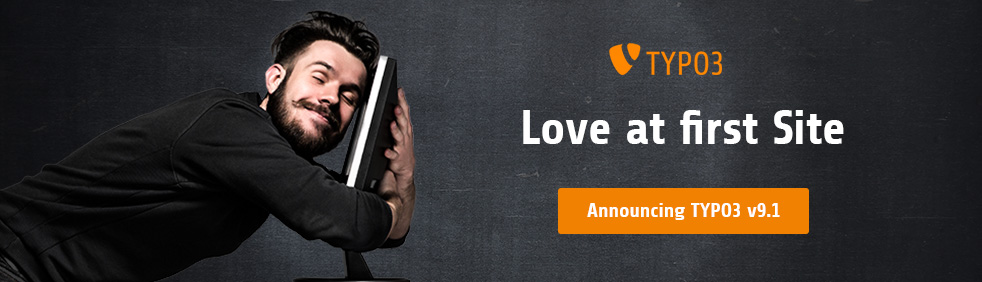
\includegraphics[width=0.95\linewidth]{Introduction/typo3-v91-banner.jpg}
	\end{figure}

\end{frame}

% ------------------------------------------------------------------------------
% LTXE-SLIDE-START
% LTXE-SLIDE-UID:		57dc32f5-8da92ccd-396fb622-361732da
% LTXE-SLIDE-ORIGIN:	baf0e8fa-b8335fbe-911020ab-489d6156 English
% LTXE-SLIDE-TITLE:		System Requirements
% ------------------------------------------------------------------------------
\begin{frame}[fragile]
	\frametitle{Introduzione}
	\framesubtitle{Requisiti di sistema}

	\begin{itemize}
		\item PHP versione 7.2\newline
			\smaller
				(potrebbe essere ridotto a PHP 7.1 o 7.0 nelle prossime release, in attesa di decisione)
			\normalsize

		\item Impostazioni PHP:

			\begin{itemize}
				\item \texttt{memory\_limit} >= 128M
				\item \texttt{max\_execution\_time} >= 240s
				\item \texttt{max\_input\_vars} >= 1500
				\item l'opzione di compilazione \texttt{-}\texttt{-disable-ipv6} \underline{non} deve essere usata
			\end{itemize}

		\item La maggior parte dei Database supportati da \textbf{Doctrine DBAL} funzionano anche con TYPO3.
			I DB verificati sono ad esempio:
	\end{itemize}

	\begin{figure}
		
\includegraphics[width=0.70\linewidth]{Introduction/logo-databases.png}
	\end{figure}

\end{frame}

% ------------------------------------------------------------------------------
% LTXE-SLIDE-START
% LTXE-SLIDE-UID:		e2edf84d-33354feb-4fc3397a-57315bf9
% LTXE-SLIDE-ORIGIN:	dfe5c3a8-72a55162-da879770-778ebfec English
% LTXE-SLIDE-TITLE:		Development, Release and Maintenance Timeline
% ------------------------------------------------------------------------------
\begin{frame}[fragile]
	\frametitle{Introduzione}
	\framesubtitle{Sviluppo e tempi di rilascio}

	\textbf{TYPO3 v9}

	\begin{figure}
		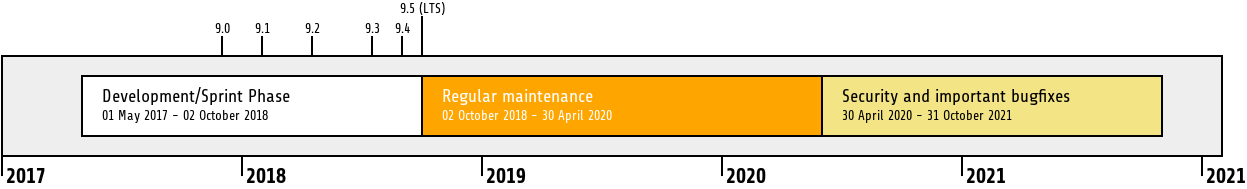
\includegraphics[width=1\linewidth]{Introduction/typo3-v9-lifecycle.png}
	\end{figure}

	\textbf{Estensione di supporto}\newline
	\smaller
		La \href{https://typo3.com}{TYPO3 GmbH} offre ulteriori opzioni di supporto
		per TYPO3 v9 LTS anche dopo il 31 ottobre 2021, per ulteriori due anni.
	\normalsize

%	\url{https://typo3.com/our-services/extended-support/}

\end{frame}

% ------------------------------------------------------------------------------
% LTXE-SLIDE-START
% LTXE-SLIDE-UID:		f55122e4-0d88bda4-809030c9-fd308c2e
% LTXE-SLIDE-ORIGIN:	1c2b096f-e4e0a65c-b0b0d84b-e18889a1 English
% LTXE-SLIDE-TITLE:		TYPO3 v9 Roadmap
% ------------------------------------------------------------------------------
\begin{frame}[fragile]
	\frametitle{Introduzione}
	\framesubtitle{TYPO3 v9 Roadmap}

	Date di rilascio stimate e loro obiettivi principali:

	\begin{itemize}

		\item v9.0 \tabto{1.1cm}12/Dic/2017\tabto{3.4cm}Install Tool e refactoring dell'albero delle pagine,\newline
			\tabto{3.4cm}Unione pagine tradotte
		\item
			\begingroup
				\color{typo3orange}
					v9.1 \tabto{1.1cm}30/Gen/2018\tabto{3.4cm}Gestione reindirizzamento
			\endgroup
		\item v9.2 \tabto{1.1cm}10/Apr/2018\tabto{3.4cm}Configurazione del sito
		\item v9.3 \tabto{1.1cm}12/Giu/2018\tabto{3.4cm}URL Routing
		\item v9.4 \tabto{1.1cm}04/Set/2018\tabto{3.4cm}Editing nel frontend
		\item v9.5 \tabto{1.1cm}02/Ott/2018\tabto{3.4cm}Rilascio LTS

	\end{itemize}

	\smaller
		\url{https://typo3.org/news/article/typo3-v9-roadmap/}
	\normalsize

\end{frame}

% ------------------------------------------------------------------------------
% LTXE-SLIDE-START
% LTXE-SLIDE-UID:		55b876ff-d5a3e107-6f7e1655-4e6b0b09
% LTXE-SLIDE-ORIGIN:	27b13d1c-5c952e3e-d4422d93-0a8a273d English
% LTXE-SLIDE-TITLE:		Installation
% ------------------------------------------------------------------------------
\begin{frame}[fragile]
	\frametitle{Introduzione}
	\framesubtitle{Installazione}

	\begin{itemize}
		\item Procedura ufficiale di installazione in Linux/Mac OS X\newline
			(Directory Root ad esempio \texttt{/var/www/site/htdocs}):
		\begin{lstlisting}
			$ cd /var/www/site
			$ wget --content-disposition get.typo3.org/9.1
			$ tar xzf typo3_src-9.1.0.tar.gz
			$ cd htdocs
			$ ln -s ../typo3_src-9.1.0 typo3_src
			$ ln -s typo3_src/index.php
			$ ln -s typo3_src/typo3
			$ touch FIRST_INSTALL
		\end{lstlisting}

		\item Link simbolici in Microsoft Windows:

			\begin{itemize}
				\item Usa \texttt{junction} in Windows XP/2000
				\item Usa \texttt{mklink} in Windows Vista e Windows 7
			\end{itemize}

	\end{itemize}
\end{frame}

% ------------------------------------------------------------------------------
% LTXE-SLIDE-START
% LTXE-SLIDE-UID:		878e2aa7-882f0ca3-c0751725-7b38e5e6
% LTXE-SLIDE-ORIGIN:	2991c08b-8831f59c-56bc188c-e05b8e92 English
% LTXE-SLIDE-TITLE:		Installation using composer
% ------------------------------------------------------------------------------
\begin{frame}[fragile]
	\frametitle{Installazione e aggiornamento}
	\framesubtitle{Installazione con \texttt{composer}}

	\begin{itemize}
		\item Installazione con \textit{composer} in Linux/Mac OS X

			\begin{lstlisting}
				$ cd /var/www/site/
				$ composer create-project typo3/minimal
			\end{lstlisting}

		\item In alternativa, create il vostro file \texttt{composer.json} ed eseguite:

			\begin{lstlisting}
				$ composer install
			\end{lstlisting}

			Un esempio di file \texttt{composer.json} può essere scaricato:\newline
			\small
				\href{https://git.typo3.org/TYPO3CMS/Distributions/Base.git/blob/HEAD:/composer.json}{git.typo3.org/TYPO3CMS/Distributions/Base.git/blob/HEAD:/composer.json}
			\normalsize

	\end{itemize}
\end{frame}

% ------------------------------------------------------------------------------
% LTXE-SLIDE-START
% LTXE-SLIDE-UID:		0cf7a1e4-1f09a2a3-5ba41749-6d82b0fe
% LTXE-SLIDE-ORIGIN:	3bc1e21e-cf2c23c4-b1d641af-8e351b92 English
% LTXE-SLIDE-TITLE:		Upgrade to TYPO3 Version 9
% ------------------------------------------------------------------------------
%\begin{frame}[fragile]
%	\frametitle{Introduction}
%	\framesubtitle{Upgrade to TYPO3 Version 9.x}
%
%	\begin{itemize}
%		\item Upgrades only possible from TYPO3 v8 LTS
%		\item TYPO3 < v8 LTS should be updated to TYPO3 v8 LTS first
%	\end{itemize}
%
%	\begin{itemize}
%
%		\item Upgrade instructions:\newline
%			\smaller\url{https://wiki.typo3.org/Upgrade#Upgrading_to_9.1}\normalsize
%		\item Official TYPO3 guide "TYPO3 Installation and Upgrading":
%			\smaller\url{https://docs.typo3.org/typo3cms/InstallationGuide}\normalsize
%		\item General approach:
%			\begin{itemize}
%				\item Check minimum system requirements \small(PHP, MySQL, etc.)
%				\item Review \textbf{deprecation\_*.log} in old TYPO3 instance
%				\item Update all extensions to the latest version
%				\item Deploy new sources and run Install Tool -> Upgrade Wizard
%				\item Review startup module for backend users (optionally)
%			\end{itemize}
%	\end{itemize}
%
%\end{frame}
%
% ------------------------------------------------------------------------------
